\documentclass{gescons}

\genre {Resumo do Biênio}
\author{Ana Claudia Prado e Magda Amancio Stapf}
\title{Gestão 2024-2025: Entrevista com as Coordenadoras}

\begin{document}
    \makeentrevistatitle
    %\maketitle

    %\fullwidthimage{fields}{b}

    %\coverart{back/editorial}
    \coverart{../fundo-generico.png}

    \begin{center}
        \noindent\includegraphics[width=14cm, height=10cm]{example-image}
    \end{center}
    
    
    \begin{multicols}{2}

%\begin{center}
%    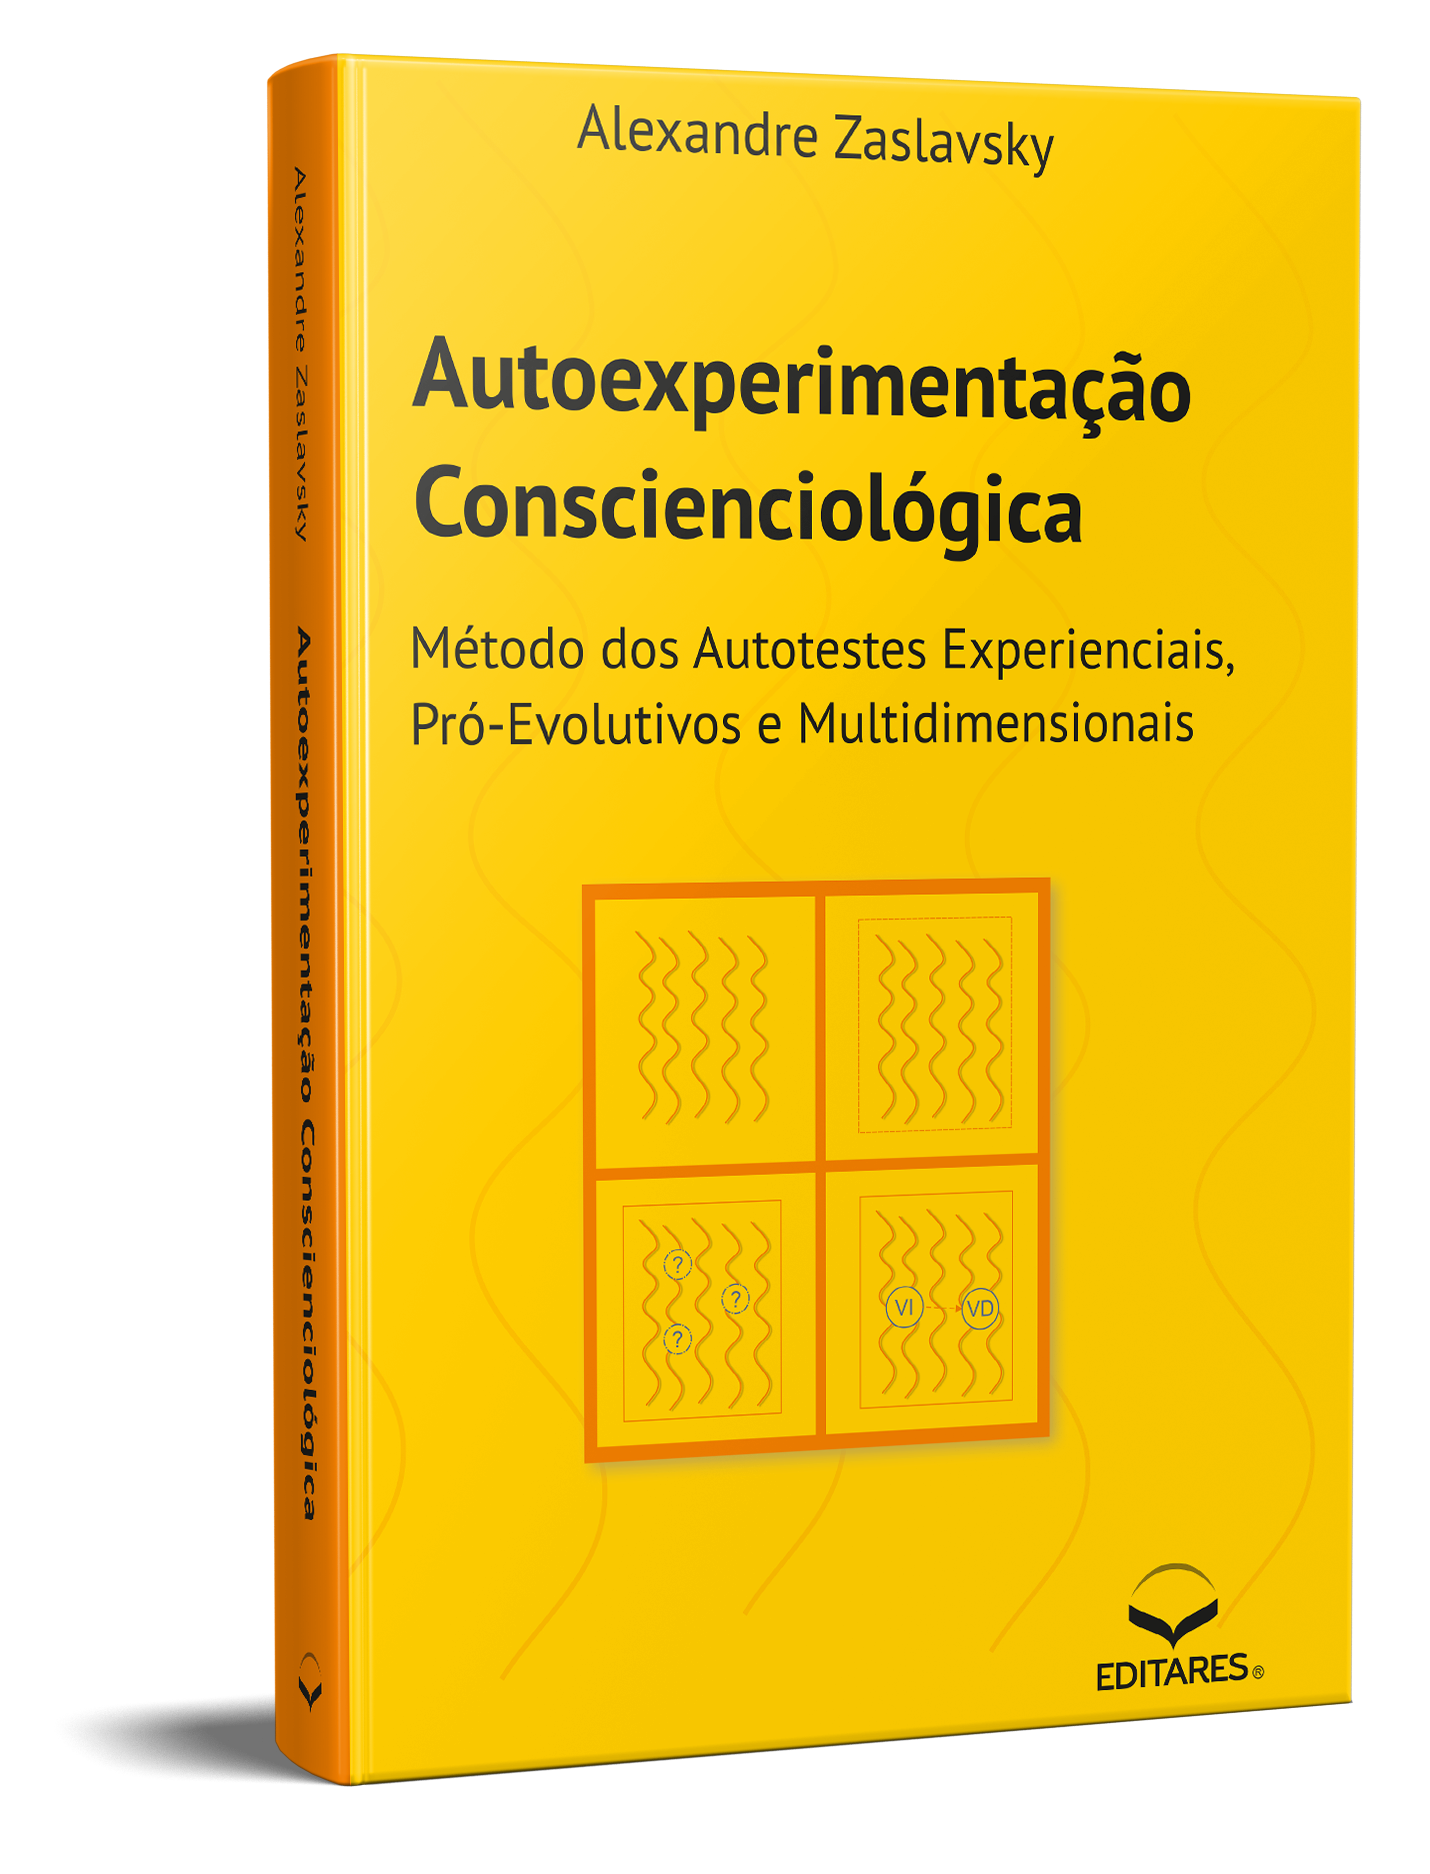
\includegraphics[width=4cm]{articles/entrevista/mockups/Alexandre-Zas.png}
%\end{center}



\textbf{Como foi o convite ou o processo de chegada de vocês à coordenação da Editares? Quais eram suas expectativas ao assumir e como elas se confirmaram ou mudaram nesses dois anos?}

\textbf{Ana:} Foi um convite bastante refletido. Precisei pensar muito antes de aceitar, porque já tinha diversas atividades. Houve um grande investimento das lideranças da Editares para que eu assumisse a coordenação, e uma das minhas condições foi que tivéssemos uma dupla. Então, convidamos a Magda.

\textbf{Magda:} Eu já tinha decidido que só toparia se fosse com a Ana. Se ela aceitasse, eu ficaria junto.

\textbf{Ana:} No início, eu não tinha muitas expectativas. As ideias foram surgindo com o tempo e fomos fazendo acontecer. Começamos organizando os contratos de cessão de direitos e planejando a mudança da sala, para acomodar melhor a equipe.

\textbf{Magda:} Eu tinha feito o curso de preparação de lideranças da Unicin, mas na época não compreendia bem o que representava. No curso, cheguei a dizer que não assumiria nenhuma gestão. Perguntaram do que eu estava me escondendo --- e essa pergunta ficou ecoando, me fazendo refletir.

\textbf{Ana:} E ainda por cima assumir a gestão da Editares, que tem uma atividade relacionada à toda CCCI. Eu também não pensava em coordenação, nem em voluntariar na Editares. Mas, ao publicar meu livro \emph{Antologia da Técnica de Mais um Ano de Vida}, senti vontade de ajudar mais, pois me identifiquei com o trabalho. Aos poucos, percebi o quanto isso se conecta com a minha proéxis: auxiliar outras pessoas a escreverem seus livros.

\begin{pullquote}
``Aos poucos, percebi o quanto isso se conecta com a minha proéxis: auxiliar outras pessoas a escreverem seus livros.''
\end{pullquote}

\textbf{Quais foram os maiores desafios enfrentados na gestão da editora nesse período? Que aprendizados pessoais e grupais vocês destacariam dessa experiência?}

\textbf{Ana:} Um dos maiores desafios foi formar equipes e reestruturar o conselho. Outro foi dar mais celeridade às publicações. Isso só foi possível graças ao envolvimento dos voluntários, autores, editores e da própria CCCI. Mostramos do que somos capazes quando trabalhamos juntos. Conseguimos organizar o fluxo de chegada das obras, fazer o acompanhamento até a publicação e manter um bom ritmo. Essa ``máquina'' só funciona porque contamos com especialistas para revisão, conferência e apoio editorial. Hoje, tudo flui bem graças ao esforço coletivo.

\textbf{Magda:} Essa experiência exigiu um amadurecimento na gestão, porque tivemos que desenvolver uma visão de conjunto. Para mim, um desafio marcante foi a quebra do sistema de gestão de estoque. Perdemos dados atualizados e tivemos que fazer um esforço enorme para recuperá-los. Trabalhei lado a lado com a Angélica {[}funcionária da Editares{]} nessa fase. A Ana estava viajando, e isso acabou ajudando, porque ela conseguia me acalmar e me manter focada na solução. Essa parceria na coordenação funcionou muito bem: quando uma estava sobrecarregada, a outra dava suporte.


\textbf{Que efeitos essa experiência trouxe para a autopesquisa e a proéxis de cada uma?}

\textbf{Ana:} Para mim, foi como se eu tivesse me localizado na proéxis. É como se tivesse feito um ``download'' não só da intermissão, mas também de experiências de outras vidas. Estar na linha de frente, na ``vitrine'', não era algo natural para mim. Aprendi a lidar com a exposição, a assumir responsabilidades e a mostrar quem eu realmente sou --- com meus traf\emph{o}res, traf\emph{a}res e traf\emph{ai}s. Um dos maiores aprendizados foi não limitar meus potenciais por medo de errar ou aparecer. Essa vivência me ajudou a superar essas barreiras internas.

\textbf{Magda:} Para mim, a gestão ampliou muito minha visão. Passei a enxergar melhor o funcionamento do grupo, amadureci e desenvolvi um senso maior de pertencimento à Comunidade Conscienciológica. Essa sensação de estar integrada e contribuir para algo maior é muito gratificante.

\textbf{Como vocês imaginam o futuro da editoração conscienciológica?}

\textbf{Ana:} Gostaria que conseguíssemos dar ainda mais celeridade às publicações. Para isso, precisamos que as obras cheguem mais bem estruturadas, o que permitiria avançar com mais rapidez. Estamos trabalhando nesse sentido.

\textbf{Magda:} As parcerias com a Uniescon podem contribuir bastante nesse processo.

\textbf{Ana:} Além disso, seria importante ampliar o engajamento de voluntários da CCCI, especialmente aqueles com disponibilidade para atuar nas revisões.

\textbf{Que mensagem final gostariam de deixar para os leitores e voluntários da Conscienciologia?}

\textbf{Ana:} Se uma oportunidade ou desafio bater à sua porta, abrace-o e leve até o fim. No final, reflita: \emph{o que aprendi com isso?}



\textbf{Magda:} Apesar dos desafios da coordenação, esse trabalho vale muito a pena. Ele contribui diretamente para o amadurecimento pessoal, grupal e intraconsciencial.

\coverart{../fundo-generico.png}

\textbf{Coordenadoras:} Agradecemos a todos os voluntários da Editares e da CCCI que contribuem e fazem parte desse trabalho interassistencial de publicação de obras conscienciológicas, ajudando a materializar as proéxis individuais e a maxiproéxis grupal!

%{[}FOTO DAS COORDENADORAS{]}



%\begin{pullquote}
%``Aos poucos, percebi o quanto isso se conecta com a minha proéxis: auxiliar outras pessoas a escreverem seus livros.''
%\end{pullquote}

        
    \end{multicols}



\begin{center}
    \noindent\includegraphics[width=14cm, height=10cm]{example-image}
\end{center}

\end{document}
